\documentclass[a4paper,12pt]{article}
\usepackage[english,russian]{babel}
\usepackage[utf8]{inputenc}
\usepackage{latexsym,mathrsfs}
\usepackage{stmaryrd, enumitem}
\usepackage{amsthm,amsfonts,amssymb,amsmath}
\usepackage{geometry}
\usepackage{tempora}
\usepackage{graphicx}
\usepackage{url}

\geometry{top=17mm}  \geometry{bottom=20mm}
\geometry{left=17mm} \geometry{right=17mm}
\linespread{1.1}
\parindent=5mm


\def\titleK#1{\begin{center}{\Large\textbf{#1}}\end{center}}
\def\authorK#1{\begin{center}{#1}\end{center}}



\newenvironment{abstractK}{}


\newtheorem{theorem}{Теорема}
\newtheorem{lemma}{Лемма}
\newtheorem{corollary}{Следствие}
\newtheorem{proposition}{Предложение}
\newtheorem{statement}{Утверждение}
\theoremstyle{definition}
\newtheorem{definition}{Определение}
\newtheorem{problem}{Задача}
\newtheorem{question}{Вопрос}
\newtheorem{conjecture}{Гипотеза}
\newtheorem{construction}{Конструкция}
\newtheorem{remark}{Замечание}

%ВАЖНО: Просьба пользоваться имеющимися окражениями-теоремами
%ВАЖНО: Не менять и не добавлять ничего выше этой строки.
%Изменения вносить только внутри окружения \begin{document}\end{document}

\begin{document}

%Название доклада
\titleK{Название тезисов}
%Информация об авторах
\authorK{И.~О.~Фамилия1$^{1}$, И.~О.~Фамилия2$^{1}$, И.~О.~Фамилия3$^{2}$\\
$^{1}$Организация Автора1 и Автора2 \\ $^{2}$Организация Автора3 \\ {\bf E-mail:} email1@g.nsu.ru, email2@g.nsu.ru, email3@gmail.com}
%Текст тезисов доклада 
%Внутри текста можно использовать стандартные команды TeX а также следующие определенные окружения
%Теорема - \begin{theorem}\end{theorem}
%Лемма - \begin{lemma}\end{lemma}
%Следствие - \begin{corollary}\end{corollary}
%Предложение - \begin{proposition}\end{proposition}
%Определение - \begin{definition}\end{definition}
%Вопрос - \begin{question}\end{question}
%Гипотеза - \begin{conjecture}\end{conjecture}
\begin{abstract}
      Аннотация. Краткое описание содержания работы. \\
\\{\bf Ключевые слова:} \textit{ ключевое слово 1, ключевое слово 2, ключевое слово 3.} 
 \end{abstract}


\begin{abstractK}

\section{Введение}

Текст введения. Если подразделы не нужны~--- то можно их не делать. Нумеровать разделы не нужно.

\section{Основная часть}

Текст тезисов.

Текст. Текст. Текст. Текст. Текст. Текст. Текст. Текст. Текст. Текст. Текст. Текст. Текст. Текст. Текст. Текст. Текст. Текст. Текст. Текст. Текст. Текст. Текст. Текст. Текст. Текст. Текст. Текст. Текст. Текст. Текст. Текст. Текст. Текст. Текст. Текст. Текст. Текст. Текст. Текст. Текст. Текст. Текст. Текст. Текст. Текст. Текст. Текст. Текст. Текст. Текст. Текст. Текст. Текст. Текст. Текст. Текст. Текст. Текст. Текст. Текст. 

Тире: ---

Неразрывные~пробелы:~по~таким~пробелам~не~будет~переноса~строки,~например,~в~этой~строчке~перенос~будет~внутри~слова.

Можно использовать стандартные команды TeX для форматирования текста. {\it Текст курсивом}. {\bf Жирный шрифт.} {\tt Шрифт печатной машинки (моноширинный)}.

Невыносные формулы в тексте: Через $\mathbb{Z}_2^n$ обозначим пространство двоичных векторов, имеющих $n$ координат. $2^{2^n}$ является очень большим числом.

Выносные формулы делаются так: полином 
$$
	f(x_1,\ldots,x_n) = \left( \bigoplus_{k=1}^{n} \bigoplus_{1 \leq i_1 < \ldots < i_k \leq n} a_{i_1,\ldots,i_k} \cdot x_{i_1}\cdot \ldots \cdot x_{i_k} \right) \oplus a_0,
$$
где $a_0, a_{i_1,\ldots,i_k} \in \mathbb{Z}_2$, называется {\it полиномом Жегалкина} ({\it алгебраической нормальной формой, АНФ)}. 

\subsection{Окружения}

Пример определения:
\begin{definition}
	Алгоритм назыается {\it эффективным}, если...
\end{definition}

Можно также уточнять определяемый объект:
\begin{definition}[Задача SVP]
	Задача... называется... и обозначается как {\it SVP}.
\end{definition}


Простые определения лучше давать в тексте: {\it Весом Хэмминга} $\mathrm{wt}(x)$ вектора $x \in \mathbb{Z}_2^n$ называется число его ненулевых координат. {\it Расстояние Хэмминга} $\mathrm{d}(x, y)$ равно $\mathrm{wt}(x \oplus y)$ для любых $x, y \in \mathbb{Z}_2^m$.

Пример теоремы:

\begin{theorem}
Текст теоремы 1.
\end{theorem}   

\begin{remark}
Теорема справедлива и для...
\end{remark}   


\subsection{Ссылки, рисунки и таблицы}

Пример ссылки на литературу: В книге~\cite{AlferovEtAl2001} приводится подробный обзор... в работе~\cite{DiffieHellman1976} предложен метод... В работе~\cite{Glukhov2013} анализируется... Ссылки на сайты \url{https://summercrypto.ru} нужно выносить в литературу и ссылаться так:~\cite{summerCryptoSite}. 

Пример ссылки на рисунок: На рис.~\ref{fig:image2} изображена...

%Пример вставки картинок
\begin{figure}[h]
\begin{minipage}[h]{0.49\linewidth}
\center{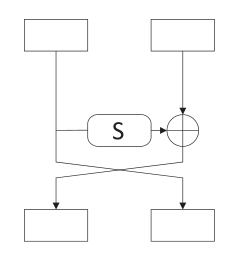
\includegraphics[width=1\linewidth]{feistel.png} }
\caption{Сеть Фейстеля}
\label{fig:image1}
\end{minipage}
\hfill
\begin{minipage}[h]{0.49\linewidth}
\center{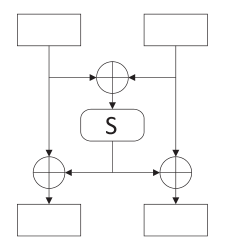
\includegraphics[width=1\linewidth]{laimassey.png} }
\caption{Схема Лая--Месси}
\label{fig:image2}
\end{minipage}
\end{figure}

\newpage
Вставка одиночного рисунка в центре: 

\begin{figure}[h]
\center{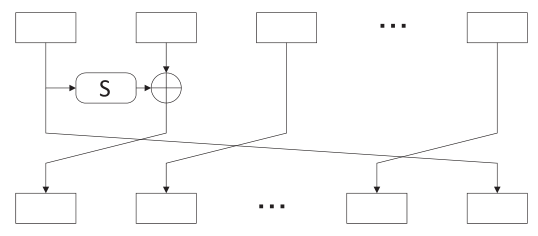
\includegraphics{gfn1.png}}
\caption{Еще схема}
\label{fig:pic3}
\end{figure}

В таблице~\ref{table:cryptosystem} приведены...

\begin{table}[h]
\centering
\begin{tabular}{|c|c|}
\hline
RSA & параметры 1\\
\hline
Classic McEliece & параметры 2\\
\hline
\end{tabular}
\caption{Параметры криптосистемы}
\label{table:cryptosystem}
\end{table} 

\section{Заключение}

В результате работы получено... Они особенно важны в контексте.... Открытыми остаются следующие вопросы...

\end{abstractK}
\renewcommand\refname{\center \textnormal{\normalsize{ЛИТЕРАТУРА}}}
%Список литературы
\begin{thebibliography}{}
    \bibitem{AlferovEtAl2001} Алферов~А.~П., Зубов~А.~Ю., Кузьмин~А.~С., Черемушкин~А.~В. Основы криптографии : учебное пособие для вузов. М. : Гелиос-АРВ, 2001.
    \bibitem{DiffieHellman1976} Diffie~W., Hellman~M.~E. New Directions in Cryptography~// IEEE Transactions on Information Theory. 1976. V.~22, I.~6. P.~644--654.
    \bibitem{Glukhov2013} Глухов~М.~М. О матрицах переходов разностей при использовании некоторых модулярных групп~// Математические вопросы криптографии. 2013. T.~4, №~4. C.~27--47.
    \bibitem{summerCryptoSite} Летняя школа по криптографии и информационной безопасности. URL: \url{https://summercrypto.ru} 
\end{thebibliography}
\bf{Кураторы исследования:} \rm{\\
 Коломеец Николай Александрович~--- к.ф.-м.н., н.с. международного научно-образовательного Математического центра НГУ;
 \\
 Куратор 2.
}
 
\end{document}